\section{Материалы предварительного проектирования системы}
\subsection{Функциональная схема обработки данных}

\begin{figure}[!htb]
    \centering
    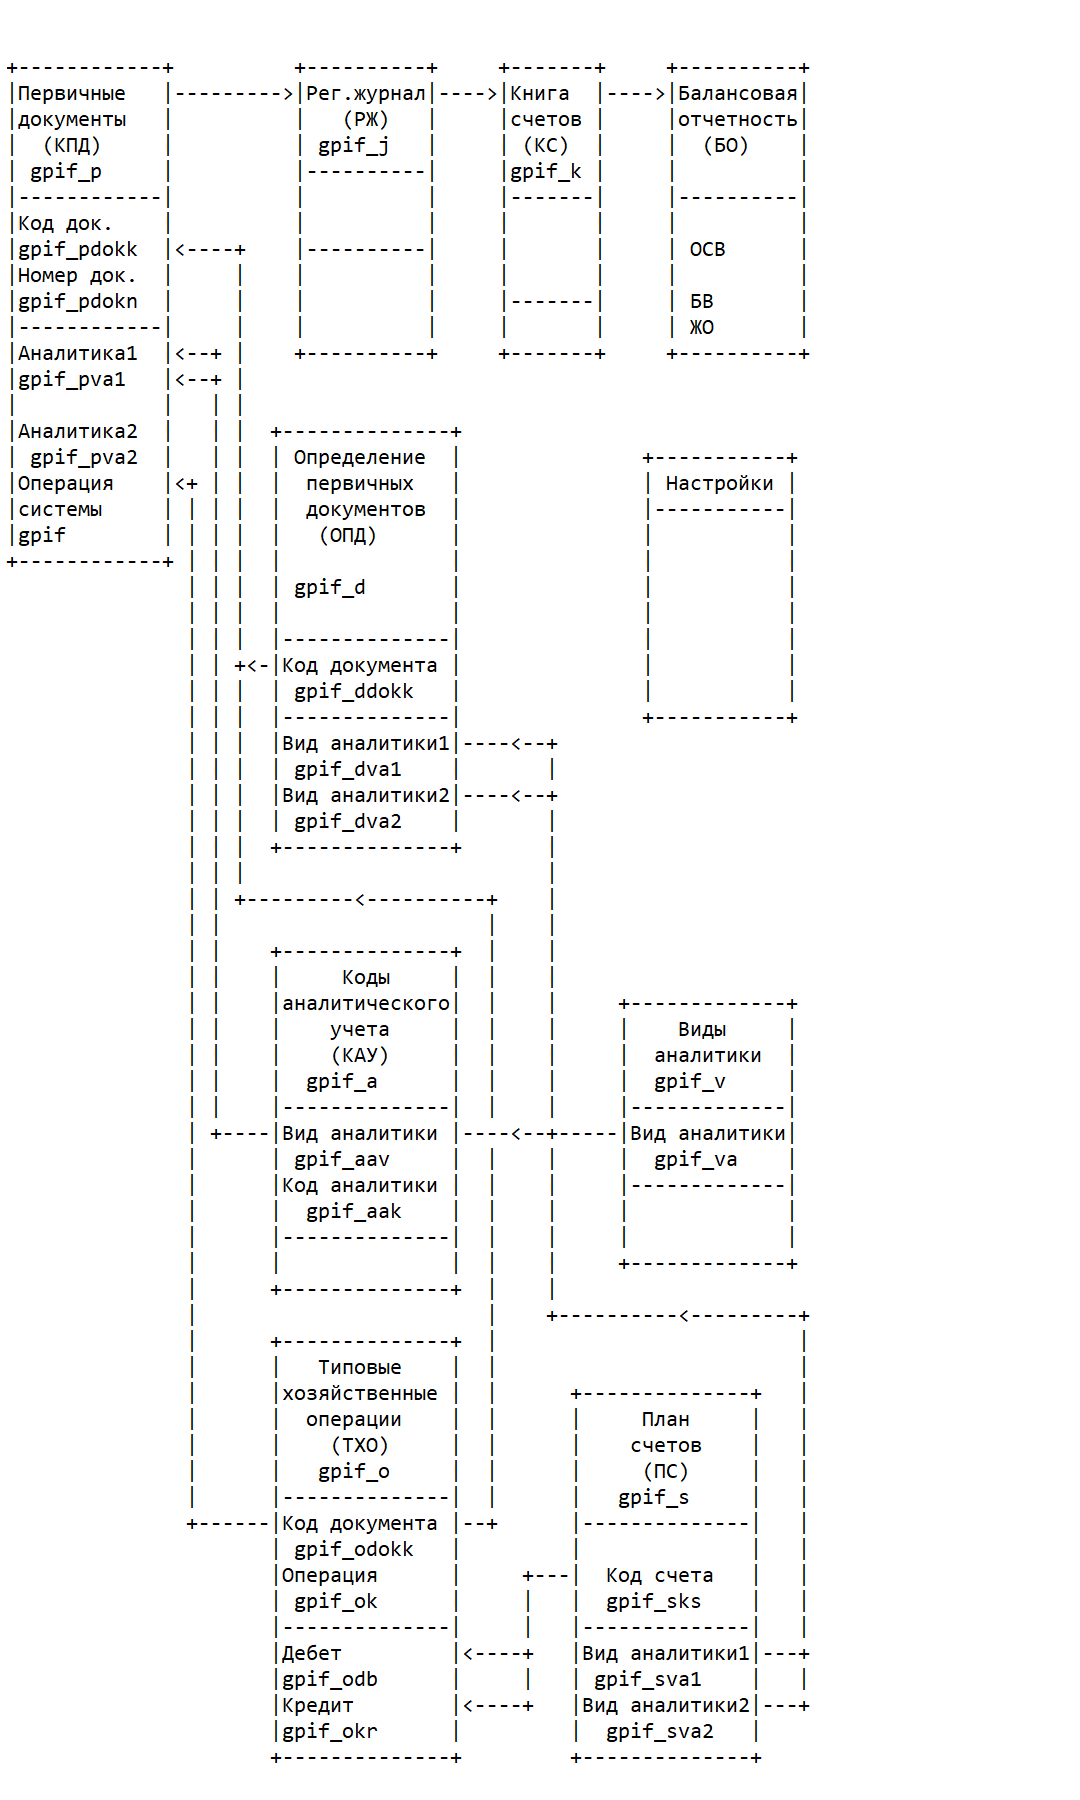
\includegraphics[height=19cm]
        {_assets/gpif_part2.png}
    \caption{Функциональная схема обработки данных}
    \label{fig:gpif_part2}
\end{figure}

\subsection{Описание картотек}

Картотеки:

\begin{itemize}
    \item Первичные документы gpif\_p;
    \item[]\hspace{0pt}
    \item Регистрационный журнал (РЖ) gpif\_j;
    \item Книга счетов (КС) gpif\_k;
    \item[]\hspace{0pt}
    \item Определение первичных документов gpif\_d;
    \item Типовые хозяйственные операции (ТХО) gpif\_o;
    \item План счетов (ПС) gpif\_s;
    \item Коды аналитического учёта (КАУ) gpif\_a;
    \item Виды аналитики gpif\_v;
    \item[]\hspace{0pt}
    \item Настройки системы gpif\_с. 
\end{itemize}

\begin{table}[h!p]
    \centering
    \scriptsize
    \caption{Первичные документы gpif\_p}
    \begin{tabular}{|l|l|l|} 

                                                                                          \hline
\textbf{Реквизит}                   &\textbf{Обозначение}   &\textbf{Тип и значность}  \\ \hline
поле связи               =0         &gpif\_p0               &n1                        \\ \hline
код документа    < --- d            &gpif\_pdokk            &c3                        \\ \hline
номер документа                     &gpif\_pdokn            &n5                        \\ \hline
дата документа                      &gpif\_pdokd            &d8                        \\ \hline
вид аналитики 1    *d               &gpif\_pav1             &c3                        \\ \hline
тип аналитики 1      =д, к, x       &gpif\_pavt1            &c1                        \\ \hline
аналитика код 1   < --- a           &gpif\_pak1             &c10                       \\ \hline
вид аналитики2                      &gpif\_pav2             &c3                        \\ \hline
тип аналитики2                      &gpif\_pavt2            &c1                        \\ \hline
аналитика код2                      &gpif\_pak2             &c10                       \\ \hline
вид аналитики3                      &gpif\_pav3             &c3                        \\ \hline
тип аналитики3                      &gpif\_pavt3            &c1                        \\ \hline
аналитика код3                      &gpif\_pak3             &c10                       \\ \hline
сумма                               &gpif\_prub             &n10                       \\ \hline
операции                            &gpif\_pto              &c10                       \\ \hline
дебет счет *o                       &gpif\_pdb              &n2                        \\ \hline
дебет счет субсчет наименование *o  &gpif\_pdbn             &c10                       \\ \hline
кредит  *o                          &gpif\_pkr              &n2                        \\ \hline
кредит название*o                   &gpif\_pkrn             &c10                       \\ \hline

    \end{tabular}
\end{table}

\begin{table}[h!p]
    \centering
    \scriptsize
    \caption{Регистрационный журнал (РЖ) gpif\_j}
    \begin{tabular}{|l|l|l|} 

                                                                                       \hline
\textbf{Реквизит}               &\textbf{Обозначение}   &\textbf{Тип и значность}   \\ \hline
поле связи	=0                  &gpif\_j0               &n1                         \\ \hline
дата операции                   &gpif\_jdata            &d8                         \\ \hline
код оправдательного документа   &gpif\_jdokk            &c3                         \\ \hline
номер документа                 &gpif\_jdokn            &n10                        \\ \hline
дата документа                  &gpif\_jdokd            &d8                         \\ \hline
содержание операции             &gpif\_jto              &c10                        \\ \hline
дебет, счет                     &gpif\_jdb              &n2                         \\ \hline
дебет, название                 &gpif\_jdbn             &c10                        \\ \hline
кредит, счет                    &gpif\_jkr              &n2                         \\ \hline
кредит название                 &gpif\_jkrn             &c10                        \\ \hline
Сумма                           &gpif\_jrub             &n10                        \\ \hline

    \end{tabular}
\end{table}

\begin{table}[h!p]
    \centering
    \scriptsize
    \caption{Книга счетов(КС) gpif\_k}
    \begin{tabular}{|l|l|l|} 

                                                                                       \hline
\textbf{Реквизит}               &\textbf{Обозначение}   &\textbf{Тип и значность}   \\ \hline
поле связи  =0                  &gpif\_k0                &n1                         \\ \hline
дата операции                   &gpif\_kdata             &d8                         \\ \hline
код оправдательного документа   &gpif\_kdokk             &c3                         \\ \hline
номер документа                 &gpif\_kdokn             &n10                        \\ \hline
дата документа                  &gpif\_kdokd             &d8                         \\ \hline
операции                        &gpif\_kto               &c10                        \\ \hline
счет                            &gpif\_ks                &n2                         \\ \hline
счёт название                   &gpif\_ksn               &c10                        \\ \hline
кор. счёт                       &gpif\_kks               &n2                         \\ \hline
кор. счет наименование          &gpif\_kksn              &c10                        \\ \hline
сумма дб                        &gpif\_kdb               &n10                        \\ \hline
сумма кр                        &gpif\_kkr               &n10                        \\ \hline

    \end{tabular}
\end{table}

\begin{table}[h!p]
    \centering
    \scriptsize
    \caption{Определение первичных документов gpif\_d}
    \begin{tabular}{|l|l|l|} 

                                                                                   \hline
\textbf{Реквизит}           &\textbf{Обозначение}   &\textbf{Тип и значность}   \\ \hline
поле связи       =0         &gpif\_d0               &n1                         \\ \hline
код документа               &gpif\_dk               &c3                         \\ \hline
наименование документа      &gpif\_dn               &c10                        \\ \hline
вид аналитики 1  < ---  v   &gpif\_dav1             &c3                         \\ \hline
тип аналитики 1    =д, к, x &gpif\_davt1            &c1                         \\ \hline
виды аналитики 2            &gpif\_dav2             &c3                         \\ \hline
тип аналитики 2             &gpif\_davt2            &c1                         \\ \hline
вид аналитики 3             &gpif\_dav3             &c3                         \\ \hline
тип аналитики 2             &gpif\_davt3            &c1                         \\ \hline

    \end{tabular}
\end{table}

\begin{table}[h!p]
    \centering
    \scriptsize
    \caption{Типовые хозяйственные операции(ТХО) gpif\_o}
    \begin{tabular}{|l|l|l|} 

                                                                                           \hline
\textbf{Реквизит}                   &\textbf{Обозначение}   &\textbf{Тип и значность}   \\ \hline
поле связи    =0                    &gpif\_o0               &n1                         \\ \hline
код документа        < ---  d       &gpif\_odok             &c3                         \\ \hline
Операции                            &gpif\_ok               &c10                        \\ \hline
дебет, счёт              < --- s\_1 &gpif\_odb              &n2                         \\ \hline
дебет, название        * s\_1       &gpif\_odbn             &c10                        \\ \hline
кредит                    < --- s\_2&gpif\_okr              &n2                         \\ \hline
кредит, название     * s\_2         &gpif\_okrn             &c10                        \\ \hline

    \end{tabular}
\end{table}

\begin{table}[h!p]
    \centering
    \scriptsize
    \caption{План счетов(ПС) gpif\_s}
    \begin{tabular}{|l|l|l|} 

                                                                                   \hline
\textbf{Реквизит}           &\textbf{Обозначение}   &\textbf{Тип и значность}   \\ \hline
поле связи        =0        &gpif\_s0               &n1                         \\ \hline
счет                        &gpif\_sk               &n2                         \\ \hline
название счета              &gpif\_sn               &c10                        \\ \hline
тип счета          = а, п, x&gpif\_styp             &c1                         \\ \hline
вид аналитики 1 из V        &gpif\_sav1             &c3                         \\ \hline
вид аналитики 2 из V        &gpif\_sav2             &c3                         \\ \hline

    \end{tabular}
\end{table}

\begin{table}[h!p]
    \centering
    \scriptsize
    \caption{Коды аналитического учёта(КАУ) gpia\_a}
    \begin{tabular}{|l|l|l|} 

                                                                               \hline
\textbf{Реквизит}       &\textbf{Обозначение}   &\textbf{Тип и значность}   \\ \hline
поле связи          =0  &gpif\_a0               &n1                         \\ \hline
вид аналитики           &gpif\_av               &c3                         \\ \hline
вид аналитики           &gpif\_ak               &c10                        \\ \hline

    \end{tabular}
\end{table}

\begin{table}[h!p]
    \centering
    \scriptsize
    \caption{Виды аналитики gpif\_v}
    \begin{tabular}{|l|l|l|} 

                                                                                   \hline
\textbf{Реквизит}           &\textbf{Обозначение}   &\textbf{Тип и значность}   \\ \hline
поле связи  	  =0        &gpif\_v0               &n1                         \\ \hline
вид аналитики               &gpif\_vk               &c3                         \\ \hline
название вида аналитики     &gpif\_vn               &c10                        \\ \hline

    \end{tabular}
\end{table}

\begin{table}[h!p]
    \centering
    \scriptsize
    \caption{Настройки системы gpia\_c}
    \begin{tabular}{|l|l|l|} 

                                                                               \hline
\textbf{Реквизит}       &\textbf{Обозначение}   &\textbf{Тип и значность}   \\ \hline
поле связи          =0  &gpif\_c0               &n1                         \\ \hline
дата текущая            &gpif\_cdatt            &d8                         \\ \hline
интервал с              &gpif\_cdats            &d8                         \\ \hline
интервал до             &gpif\_cdatd            &d8                         \\ \hline
cчёт                    &gpif\_cs               &n2                         \\ \hline
название счёта          &gpif\_csn              &c10                        \\ \hline
название фирмы          &gpif\_cfirm            &c10                        \\ \hline

    \end{tabular}
\end{table}

\newpage

\subsection{Описание работ}

\begin{table}[h!p]
    \centering
    \scriptsize
    \caption{Описание работ}
    \begin{tabular}{|p{8cm}|p{8cm}|} 

% = = = = = = = = = =

\hline

% = = = = = = = = = =

\textbf{Группа работ}
&
\textbf{Работы}
\\ \hline

% = = = = = = = = = =

Формирование и разноска первичных документов \par
\hspace{0pt} \par
\textbf{gpif\_документы}
&
- gpif\_ввод текущей даты \par
- gpif\_ввод и разноска первичных документов
\\ \hline

% = = = = = = = = = =

Работа с регистрационным журналом \par
\hspace{0pt} \par
\textbf{gpif\_РЖ}
&
- gpif\_просмотр РЖ \par
- gpif\_формирование КС и РЖ \par
- gpif\_просмотр КС \par
- gpif\_сформировать КС на печать \par
- gpif\_просмотр КС для печати
\\ \hline

% = = = = = = = = = =

Формирование балансовой отчетности \par
\hspace{0pt} \par
\textbf{gpif\_БО}
&
- gpif\_опеделение отчетных форм \par
- gpif\_сформировать КС на печать \par
- gpif\_просмотр КС для печати \par
- gpif\_сформировать ОСВ \par
- gpif\_просмотр ОСВ \par
- gpif\_сформировать Ж-О \par
- gpif\_просмотр Ж-О \par
- gpif\_сформировать БВ \par
- gpif\_просмотр БВ
\\ \hline

% = = = = = = = = = =

Сопровождение картотек-справочников \par
\hspace{0pt} \par
\textbf{gpif\_картотеки}
&
- gpif\_определение первичных документов \par
- gpif\_типовые хозяйственные операции (ТХО) \par  
- gpif\_план счетов (ПС) \par
- gpif\_виды аналитики \par 
- gpif\_коды аналитического учёта (КАУ) \par
- gpif\_настройка АРМа
\\ \hline

% = = = = = = = = = =

Ведение архивов \par
\hspace{0pt} \par
\textbf{gpif\_архив}
&
- gpif\_копия АРМ \par
- gpif\_восстановление АРМ 
\\ \hline

% = = = = = = = = = =

    \end{tabular}
\end{table}

\newpage
